\documentclass[11pt]{article}
\usepackage{graphicx}
\marginparwidth 0pt
\oddsidemargin  0pt
\evensidemargin  0pt
\marginparsep 0pt
\usepackage{amsmath}
\topmargin 0pt
\usepackage{mathtools}
\textwidth   6.5 in
 \textheight  8 in
\usepackage{fancyhdr}
\renewcommand{\headrulewidth}{2pt}
\renewcommand{\footrulewidth}{1pt}
 
\pagestyle{fancy}
\usepackage{amsmath}
 %%%%%%% %%%%%%% %%%%%%% %%%%%%% %%%%%%% %%%%%%%For python%%%
 % Default fixed font does not support bold face
\DeclareFixedFont{\ttb}{T1}{txtt}{bx}{n}{12} % for bold
\DeclareFixedFont{\ttm}{T1}{txtt}{m}{n}{12}  % for normal

% Custom colors
\usepackage{color}
\definecolor{deepblue}{rgb}{0,0,0.5}
\definecolor{deepred}{rgb}{0.6,0,0}
\definecolor{deepgreen}{rgb}{0,0.5,0}

\usepackage{listings}

% Python style for highlighting
\newcommand\pythonstyle{\lstset{
language=Python,
breaklines=true,
basicstyle=\ttm,
otherkeywords={self},             % Add keywords here
keywordstyle=\ttb\color{deepblue},
emph={MyClass,__init__},          % Custom highlighting
emphstyle=\ttb\color{deepred},    % Custom highlighting style
stringstyle=\color{deepgreen},
frame=tb,                         % Any extra options here
showstringspaces=false            % 
}}

%++++++Hyperlink
\usepackage{hyperref}
\hypersetup{
    colorlinks=true,
    linkcolor=blue,
    filecolor=magenta,      
    urlcolor=cyan,
}

%%For table
\usepackage{array}
\newcolumntype{L}[1]{>{\raggedright\let\newline\\\arraybackslash\hspace{0pt}}m{#1}}
\newcolumntype{C}[1]{>{\centering\let\newline\\\arraybackslash\hspace{0pt}}m{#1}}
\newcolumntype{R}[1]{>{\raggedleft\let\newline\\\arraybackslash\hspace{0pt}}m{#1}}




% Python environment
\lstnewenvironment{python}[1][]
{
\pythonstyle
\lstset{#1}
}
{}

% Python for external files
\newcommand\pythonexternal[2][]{{
\pythonstyle
\lstinputlisting[#1]{#2}}}

% Python for inline
\newcommand\pythoninline[1]{{\pythonstyle\lstinline!#1!}}
%%%%%%%%%%%%%%%%%%%%%%%%%%%%%%%% %%%%%%% %%%%%%% %%%%%%%


%\pagestyle{empty}

\begin{document}


\begin{center}
  {\bf
  CS 534 Machine Learning  }

\vspace{12pt}

  Project 3, due Sunday, April 15
  \\
  Chenxi Cai \\
  Yifei Ren \\
  Qingfeng (Kee) Wang
 
\end{center}

\vspace{12pt}




\clearpage
(Notice, all links (table of contents, figures references, table references etc.) are clickable! You can download this PDF and open it using Preview or Adobe Reader to enable this convenient feature.)
 
\tableofcontents{}

\clearpage


\section{Introduction}
Convolutional neural network (CNN) proves to be one of the most successful training models. This time we will use CNN to train MNIST data. MNIST is a database of handwritten figures in black and white. It contains 55000 training images and 10000 test images. In this report, we split 55000 training data into 80\% data for training and 20\% for validation. We first construct a base model and then 

After adjusted some hyper-parameters, we are going to choose the parameters that gives the best validation accuracy and lowest loss. 

Then adjustment of hyper-parameters contains two stages. We first construct a base model with certain hyper-parameter.



\section{Adjust hyper-parameters I}
In this section we first adjust several hyper-parameters listed in the requirement 2.


\subsection{Size of the filters}
In basis model, size of filters is 5-by-5. According to Stanford University video courses lecture 5, common settings of filter size are listed in the Table \ref{tab:fsp}.






\begin{table}[!htb]
\centering
\caption{Commonly adjusted filter sizes. Where F is filters' spatial extend (filter dimension), S is the stride, P is the amount of zero padding. 
}
\label{tab:fsp}
\begin{tabular}{C{3cm} C{3cm} C{3cm}}
\hline \hline

F	&S	&P		 \\ \hline 
3	&1	&1 \\
5	&1	&2 \\
1	&1	&0 \\ \hline \hline

\end{tabular}
\end{table}

Here we tried three different cases of filter's size: 1*1, 3*3 and 5*5. The plot of accuracy showed in Tensorboard is listed below:

Now we know that the final accuracy after 5000 steps are shown in Table \ref{tab:filter}.

\begin{table}[!htb]
\centering
\caption{Accuracy of 5000 steps }
\label{tab:filter}
\begin{tabular}{C{5cm} C{2cm} C{2cm} C{2cm}}
\hline \hline

Size of filters	&1-by-1	&3-by-3	&5-by-5		 \\ \hline  
Accuracy	&0.7676	&0.9133	&0.9252 \\ \hline \hline

\end{tabular}
\end{table}

\subsection{Number of filters}
In basis model, filter number is 32 for conv 1 and 64 for conv 2. According to Stanford University video courses lecture 5, common settings of filter number are power of 2: 32, 64, 128 and 512, etc.
Here we tried four different cases of filter?s number (conv1, conv2): (32,32), (32,64), (64,64) and (128,128). The plot of accuracy showed in tensorboard is listed below:
\\
(pictures)
\\
Now we know that the final accuracy after 5000 steps are shown in Table  \ref{tab:num-filter}.

\begin{table}[!htb]
\centering
\caption{Validation ccuracy at 5000 steps}
\label{tab:num-filter}
\begin{tabular}{C{6cm} C{2cm} C{2cm} C{2cm} C{2cm}}
\hline \hline

Number of filter (conv1, conv2)	&(32,32)	&(32,64)	&(64,64)	&(128,128)		 \\ \hline
Accuracy at 500 step  	&0.3860	&0.4485	&0.6018	&0.4367 \\
Accuracy at 5000 step	&0.9221	&0.9133	&0.9268	&0.9253 \\ \hline \hline
\end{tabular}
\end{table}


From the table, the accuracy increases little with number, the final accuracies are very close. However, from the accuracy plots, we ca see that the initial accuracies at 500 steps have large differences:
\begin{figure}[!htb]
   \centering
   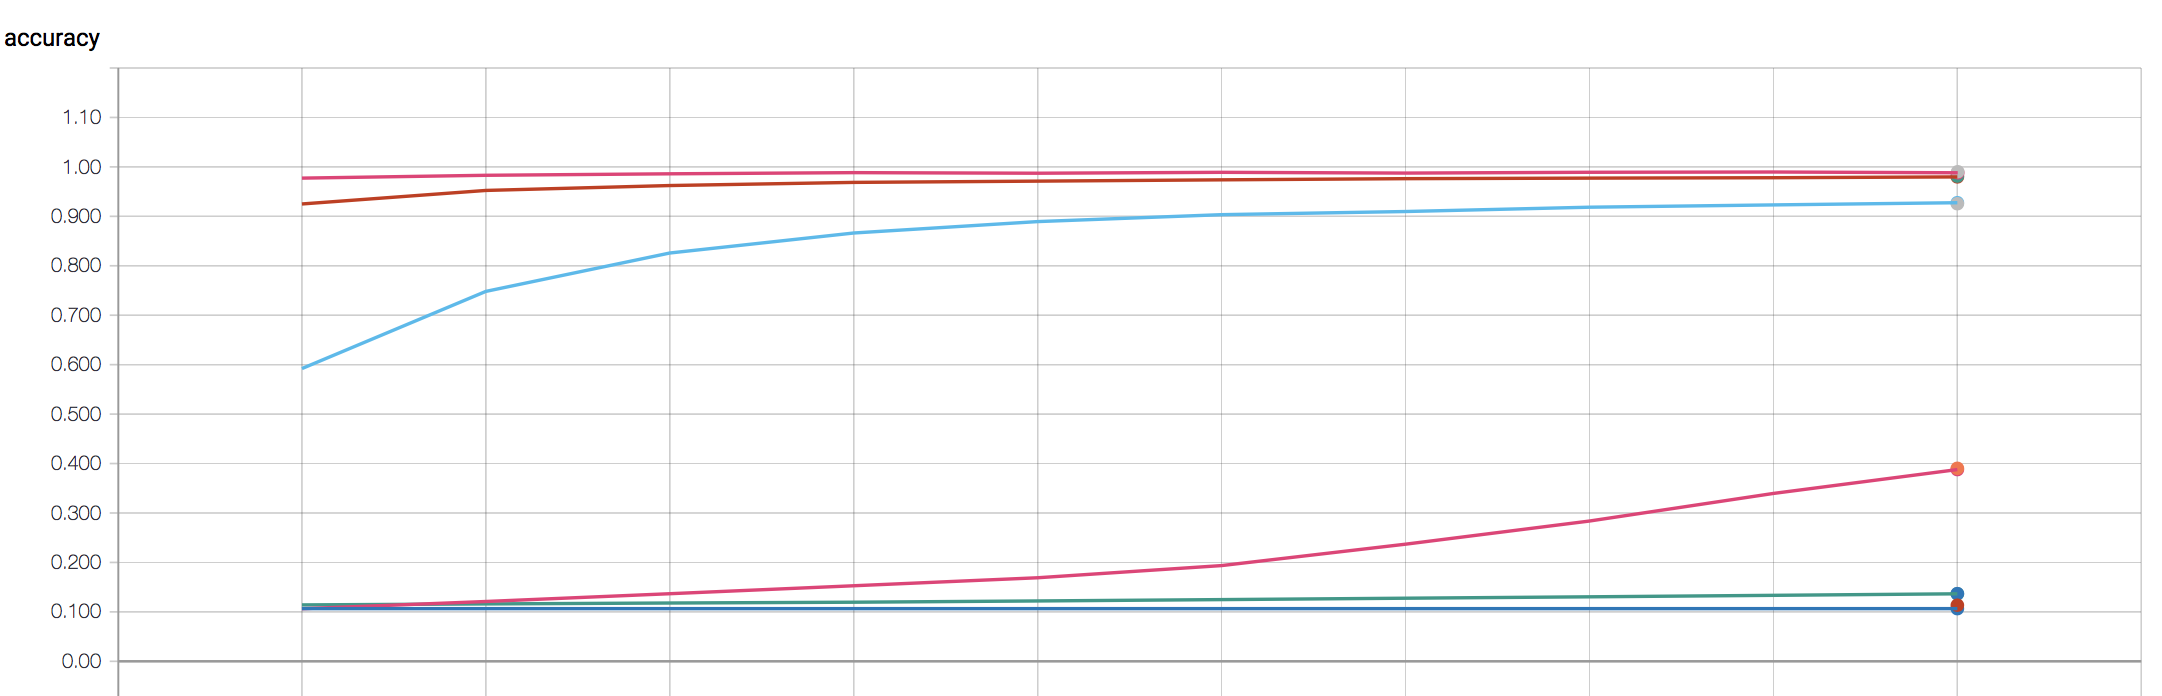
\includegraphics[width=16cm]{images/test.png} % requires the graphicx package
   \caption{example caption}
   \label{fig:example}
\end{figure}



\subsection{Number of convolution and pooling layers}

The structure of base model contains 2 convolutional layers and 2 pooling layers, shown in Figure \ref{fig:2-c-2-p}.

\begin{figure}[!htb]
   \centering
   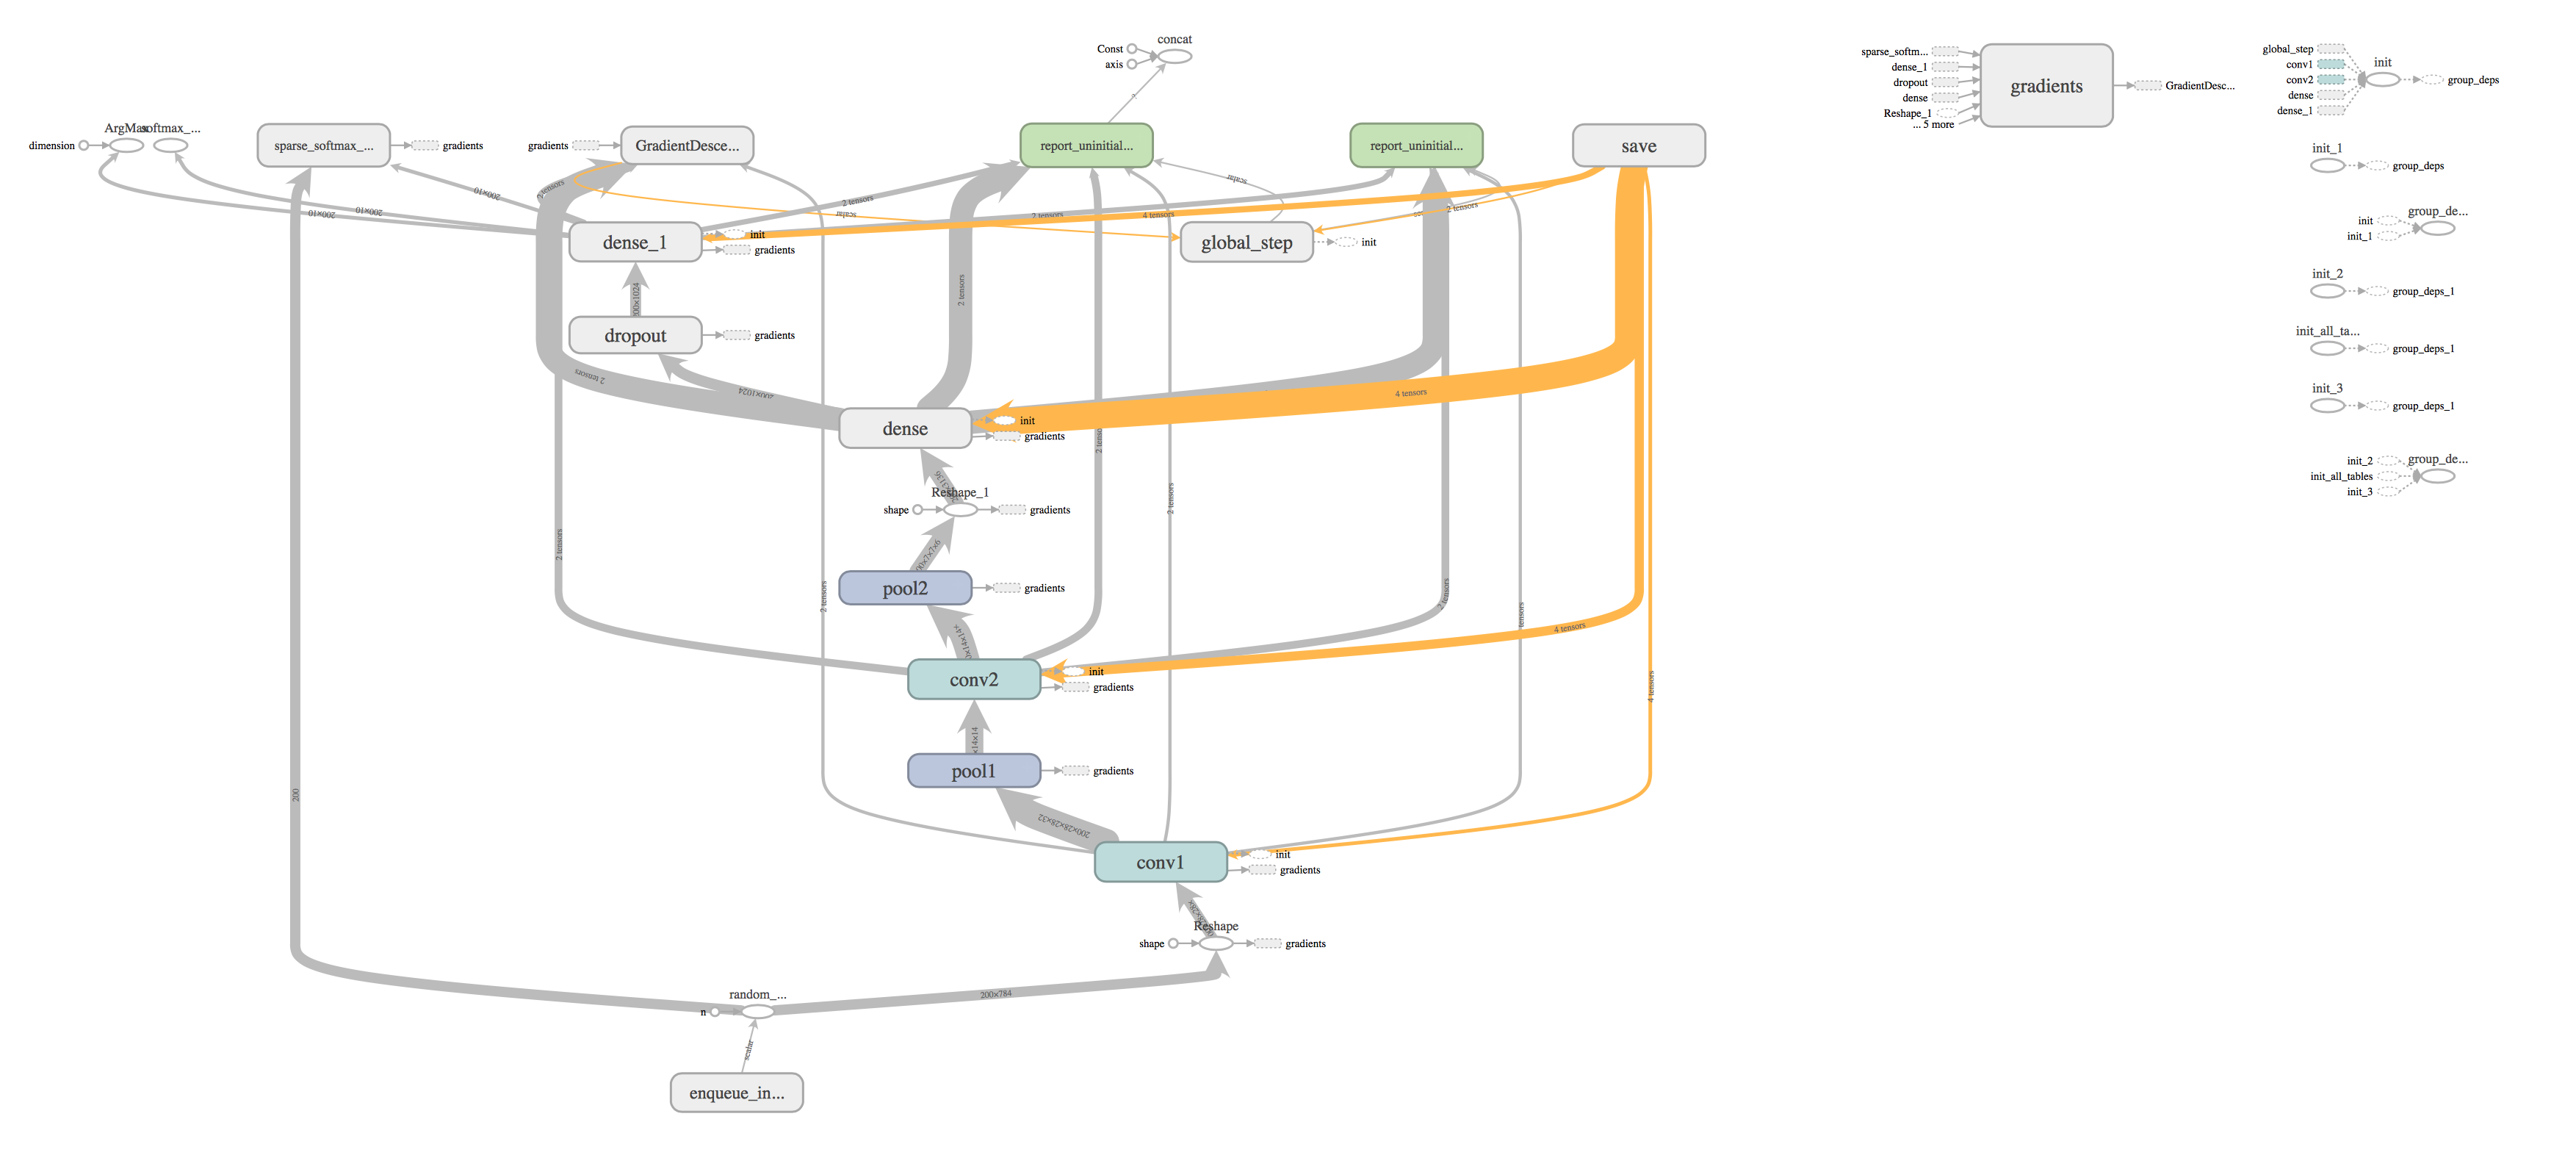
\includegraphics[width=16cm]{images/graph.png} % requires the graphicx package
   \caption{Zoom in to see details.}
   \label{fig:2-c-2-p}
\end{figure}





\clearpage
\section{Finally model and summary}





\clearpage
\section{Source codes}

Finally, codes are enclosed here.

\pythonexternal{./../project3.py}




\vspace{24pt}



\end{document}


